\section{Experimental Results}
\label{sec:exp}
\subsection{Experimental Setup}
Our application is running on EC2 instances. 
For all our experiments we used t1.micro instances but found out that it cannot service more than 10 requests and cannot cope with bursts of traffic\footnote{http://docs.amazonwebservices.com/AWSEC2/latest/UserGuide/concepts\_micro\_instances.html}. 
We were using t1.micro as it is part of AWS free tier group. 
So if the company anticipates say 100 users at a time, then they need 10 t1.micro instances and scale up or down accordingly.
Hence, we use the next instance type m1.small for our application. 
The auto-scaling system implementation will only  spawn m1.small instances as new instances. 
For testing each module of the system design, we developed simple python scripts which use threads. 
We use a 105KB file that will be converted to the desired format. 
The IaaS system also runs on a python script which uses boto to interface with the AWS.

\subsection{Experiments}
All the experiments test the automation and monitoring features of the system, we run the IaaS system scripts and then experiment scripts, thus automating the whole process. 
Monitoring is being done for every instance, by default we start detailed monitoring on each newly launched instance and stores the output in a log file.
\subsubsection{Experiment 1}
\paragraph{Objective}
For the first experiment we test our application with 100 concurrent client requests without our IaaS system. 
we launched 100 threads that individually made concurrent client requests. 
\paragraph{Analysis}
We get a server error, which means that a single m1.small instance cannot handle 100 concurrent requests.
Figure \ref{fig:noscaling} displays the CPU utilization for a certain time span of the cloud based system without auto scaling.
As can be seen from the figure the instance reaches 100 percent CPU-utilization and cannot service any additional client request.    

\begin{figure}[h]
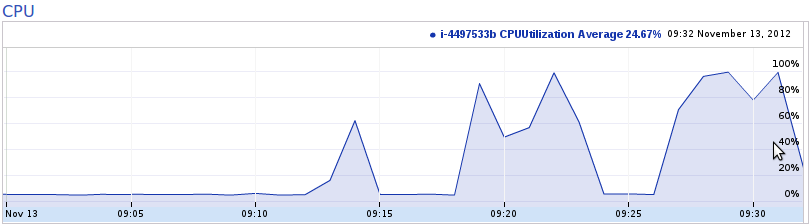
\includegraphics[scale=0.695]{noscaling.png}
\caption{Cloud based system working without auto-scaling}
\label{fig:noscaling}
\end{figure}

\subsubsection{Experiment 2}
\paragraph{Objective}
We want to test the security of the application by implementing security groups. 
We create a security group through our system script with only 80(HTTP) port and launch our instances attached to that security group. 
Next we try to SSH to the instance using the keypair we generated from AWS.
\paragraph{Analysis}
We are not able to SSH into the instance and it shows an authentication error, this is because the instance is not deployed with a keypair and the security group doesn�t allow us to use SSH port of the instance.
\subsubsection{Experiment 3}
\paragraph{Objective}
Our last experiment consists of testing our application with IaaS implementation of autoscaling and load balancing. For this we write a script that runs 60 threads at a gap of 30 seconds between the starting time of the batch. 
We set the upper CPU threshold parameter to 75 percent. 
The execution should cause the system to spawn a new instance when the average CPU utilization for the past one minute goes beyond 75 percent.
\paragraph{Analysis}
As this experiment can be seen as a scenario when the application is catering to 60 concurrent users every 30 seconds. 
We noted the response times for 20,40 and 60 concurrent users, and observed that if the number of concurrent users increase the server response time increases and users might have to wait for the converted video file.
Figure \ref{fig:instance1}, \ref{fig:instance2} and \ref{fig:instance3} shows the CPU utilization during a certain time span of the three created instances with the aid of auto-scaling and load-balancing  

\subparagraph{Charged-time and charged-cost} for this experiment the load increases gradually new instances are spawned and application works with 3 instances for close to 15 mins, this can be extrapolated to an hour.

\[
charge time per hour = 3 * m1.small pricing = 3 * \$0.065 =
\$ 0.195
\]

The aforementioned equation is the charge time per hour for 60 users.
\begin{figure}[h]
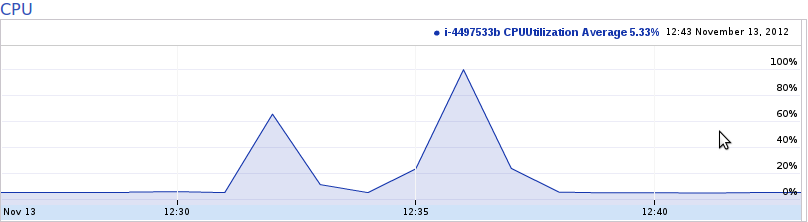
\includegraphics[scale=0.695]{instance1.png}
\caption{CPU utilization of original instance}
\label{fig:instance1}
\end{figure}

\begin{figure}[h]
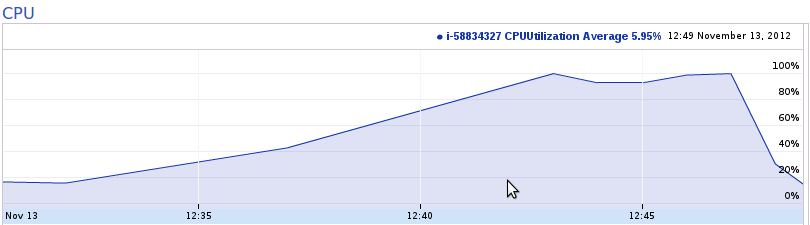
\includegraphics[scale=0.695]{instance2.png}
\caption{CPU utilization instance created by cloud based system using auto-scaling}
\label{fig:instance2}
\end{figure}

\begin{figure}[h]
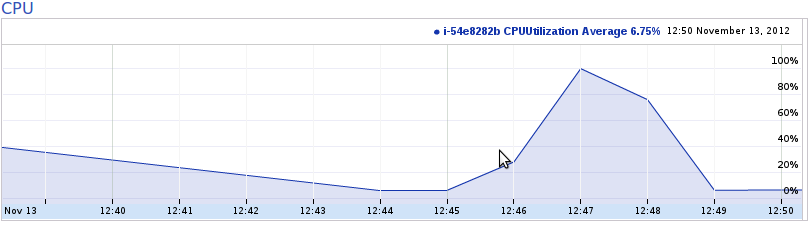
\includegraphics[scale=0.695]{instance3.png}
\caption{CPU utilization Second instance created by cloud based system using auto-scaling}
\label{fig:instance3}
\end{figure}